\chapter{Analysis and Specification of Needs}

\section{Introduction}

In this chapter, we will present the analysis and specification of needs. We start by presenting the specification of the requirements, illustrating them using the diagram of the global use cases. Then we will present our project architecture and our working environment, and finally we will present our product backlog and releases planning, and we will close our chapter with a conclusion.

\section{Requirements Specification}

In this section, we will define the actors of our application and the functional and non-functional needs that our application aims to fulfill.

\subsection{Identifying Actors}

We define actors as a shorthand for the roles played by entities outside the system that interact directly with them. In our system, we identify four types of actors:

\begin{itemize}
    \item \textbf{\textcolor{primary}{Super Admin}}: Responsible for the global configuration of the platform, they have extended privileges to manage administrators, oversee security, and ensure compliance. They can also configure advanced features and control all system resources.
    
    \item \textbf{\textcolor{primary}{Admin}}: In charge of the day-to-day management of the platform, they can add, modify, or delete listings, supervise agency and user profiles, and ensure smooth operations. They are also responsible for monitoring and assisting other actors.
    
    \item \textbf{\textcolor{primary}{Real Estate Agent}}: Dedicated to creating and updating real estate listings, they manage property information, handle investor requests, and finalize transactions related to sales or rentals. They can also coordinate property visits and propose tailored offers.
    
    \item \textbf{\textcolor{primary}{Investor}}: A user who wishes to browse and finance real estate projects. They have access to all available offers, can make investments in a few simple steps, and monitor the evolution of their portfolio. They also benefit from personalized insights to optimize their investments.
    
    \item \textbf{\textcolor{primary}{System}}: The entity that automatically manages all basic functionalities, such as authentication, notification generation, transaction validation, and adherence to security protocols. It ensures the coherence and reliability of the application at all times.
\end{itemize} 

\subsection{Functional Requirements}

After several meetings with our client, the various functional requirements of our application are illustrated as follows:

\subsubsection{For the Super Admin (Korpor)}
\begin{itemize}
    \item \textbf{Authenticate}: The super admin enters their credentials to access the advanced management console.
    \item \textbf{Log Out}: After viewing or updating global settings, they can securely log out.
    \item \textbf{Manage Admin Accounts}: Create, enable/disable, or modify admin profiles associated with different real estate companies.
    \item \textbf{Monitor Security \& Compliance}: Oversee transactions, data integrity, and regulatory adherence using specialized reporting and audit tools.
    \item \textbf{Configure Platform Features}: Define key parameters (payment methods, AI/blockchain integrations, etc.) and roll out feature updates.
    \item \textbf{View Global Reports}: Generate and analyze consolidated metrics (financials, user activity, transactions) for overall performance insights.
    \item \textbf{Moderate Content}: Review and remove any inappropriate or erroneous property listings or user-generated data.
\end{itemize} 

\subsubsection{For the Admin (Real Estate Company)}
\begin{itemize}
    \item \textbf{Authenticate}: The admin logs in with valid credentials to manage daily operations.
    \item \textbf{Log Out}: They can end their session to maintain account security.
    \item \textbf{Manage Real Estate Listings}: Add, update, or delete property listings visible to investors.
    \item \textbf{Oversee Real Estate Agents}: Create and manage agent accounts, assign properties, and monitor performance and commissions.
    \item \textbf{Track Transactions \& Commissions}: Review incoming payments, calculate commissions owed to agents, and track the history of completed deals.
    \item \textbf{Address Investor Inquiries}: Respond to questions or concerns from investors, ensuring a smooth user experience.
    \item \textbf{Access Agency Dashboard}: View comprehensive statistics on properties, sales, rentals, and market trends.
\end{itemize}

\subsubsection{For the Real Estate Agent}
\begin{itemize}
    \item \textbf{Authenticate}: The agent logs in to manage assigned properties and interact with potential investors.
    \item \textbf{Log Out}: Securely exit the account after completing tasks.
    \item \textbf{Manage Assigned Properties}: Create new listings, update property details, set prices, and upload images.
    \item \textbf{Handle Investment Requests}: Review purchase or rental offers, negotiate terms, and initiate contract finalization.
    \item \textbf{Contribute to AI Estimates}: Provide or refine data to improve AI-driven pricing and market analysis.
    \item \textbf{Maintain Client Relationships}: Communicate with investors, schedule property visits, and follow up on inquiries.
    \item \textbf{View Commissions}: Track earnings based on successful sales or rentals.
\end{itemize}

\subsubsection{For the Investor (Mobile App User)}
\begin{itemize}
    \item \textbf{Create an account \& authenticate}: Register to gain access to the platform's core features.
    \item \textbf{Log Out}: End the session to protect personal and financial data.
    \item \textbf{Browse Listings \& Invest}: Explore available properties, filter according to preferences, and commit to an investment in a few steps.
    \item \textbf{Track Portfolio}: Monitor owned assets, property status, and receive real-time updates on performance.
    \item \textbf{Make Payments}: Use integrated payment methods (credit cards, digital wallets, etc.) to complete transactions.
    \item \textbf{Access AI Recommendations}: View data-driven insights and return-on-investment estimates generated by the system.
    \item \textbf{Manage Withdrawals \& Earnings}: Withdraw profits, monitor rental income, or exit investments under the right conditions.
\end{itemize}

\subsubsection{For the System}
\begin{itemize}
    \item \textbf{Automate Authentication}: Validate credentials, manage sessions, and maintain user roles and permissions.
    \item \textbf{Generate Notifications}: Send real-time alerts (e.g., new listings, completed transactions, commission updates) to relevant users.
    \item \textbf{Ensure Compliance \& Security}: Leverage blockchain for data integrity, verify payments, and detect anomalies or fraudulent activities.
    \item \textbf{Coordinate AI Insights}: Aggregate and analyze real estate data to produce market predictions and price recommendations.
    \item \textbf{Maintain Transaction Consistency}: Update dashboards, user balances, and property statuses automatically upon each operation.
    \item \textbf{Optimize Performance}: Monitor server load, scale resources, and ensure a smooth, responsive application experience.
\end{itemize} 

\subsection{Non-functional Requirements}

In order to ensure the proper functioning of the decision-making system and to avoid any kind of anomaly, the implemented solution must meet a set of non-functional needs such as:

\begin{itemize}
    \item \textbf{Maintainability}: The system must be designed for simplicity so that tasks, updates, and bug fixes can be executed with minimal complexity.
    
    \item \textbf{Evolution}: Platform administration must remain attentive to user needs and feedback, continuously enhancing the services offered while preserving the application's utility and efficiency.
    
    \item \textbf{Security}: Robust security measures are essential. The platform must enforce strong authentication protocols, access privileges, and comprehensive data encryption (both at rest and in transit). The integration of blockchain technology further ensures the immutability and integrity of sensitive information.
    
    \item \textbf{Efficiency}: The application must be effective in all circumstances, delivering prompt and reliable functionality regardless of external conditions.
    
    \item \textbf{Performance}: The system must operate optimally across diverse environments. It should consistently provide a responsive and reliable experience, even under high transaction volumes or varying network conditions.
\end{itemize} 

\section{Requirements Analysis}

In this section, we'll outline the various features that our app should offer, using a general use case diagram.

\subsection{General use case diagram}

Below, we present the various actors of the application and the actions they are authorized to perform.
The overall diagram is illustrated in the following figure:

\begin{figure}[htbp]
    \centering
    % Replace with actual image file once available
    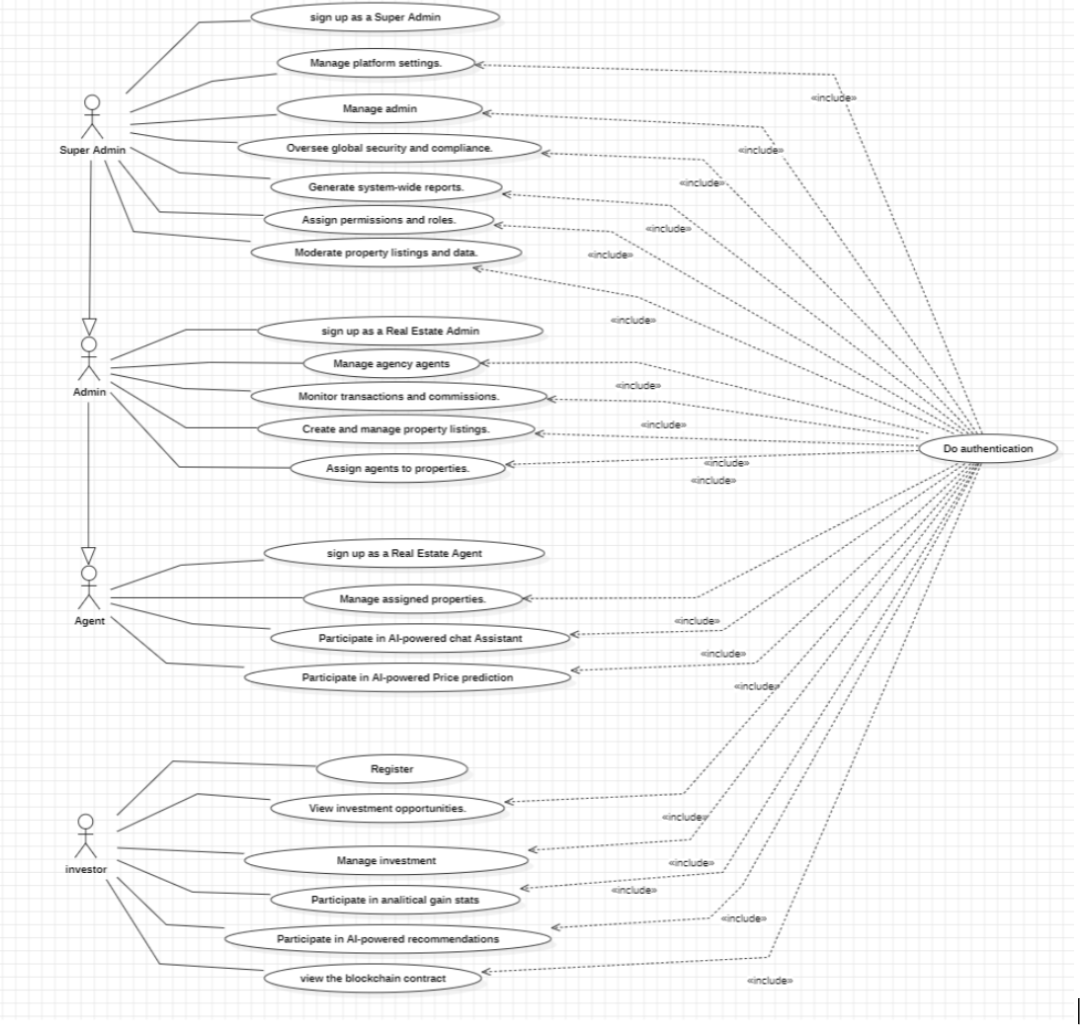
\includegraphics[width=0.85\textwidth]{images/diagram de case d utilisation general.png}
    \caption{General use case diagram}
    \label{fig:use-case-diagram}
\end{figure}

\section{Software architecture}

Before starting the design and development of any computerized system, it is essential to prepare the architecture.

\subsection{Physical architecture}

 The physical architecture of Korpor leverages modern, scalable technologies to deliver a seamless investment platform. The frontend is built with Expo, React, and TypeScript using Vite for rapid development and Tanstack for robust state management and data visualization, while Storybook supports isolated UI component development. The backend relies on Express.js with user authentication managed by Clerk, containerization via Docker, and MySQL for data storage hosted on Microsoft Azure. Integrated AI modules provide personalized insights, and blockchain technology ensures transactional security and data immutability. This setup is further supported by GitHub for version control, Postman for API testing, and end-to-end testing tools like Maestro and Playwright, with architectural designs and documentation maintained using StarUML and Overleaf.

\begin{figure}[htbp]
    \centering
    % Replace with actual image file once available
    % \includegraphics[width=0.85\textwidth]{images/physical_architecture.png}
    \caption{Physical architecture}
    \label{fig:physical-architecture}
\end{figure}

\subsection{Logical architecture}

The logical architecture of Korpor is structured around a modular, API-driven design, ensuring clear separation of concerns, scalability, and maintainability. The system follows a Model-View-Controller (MVC) approach, where each component has a distinct responsibility in managing data flow and user interactions.

Architecture Components:
\begin{itemize}
    \item \textbf{Model:} The MySQL database serves as the core data source, responsible for storing and managing application data, including user profiles, real estate listings, transactions, and investment records. The data layer interacts with the backend through ORM or query-based operations, ensuring efficient data retrieval and persistence.
    
    \item \textbf{Controller:} The Express.js backend acts as the intermediary between the database and the frontend, handling user requests, business logic, and data validation. It processes API calls from the frontend and interacts with services such as Clerk for authentication, AI modules for predictive analytics, and blockchain integration for secure transactions.
    
    \item \textbf{View:} The frontend is built with React, TypeScript, and TanStack tools, ensuring a responsive and interactive UI. The frontend communicates with the backend via API requests, displaying dynamic content and allowing seamless user interaction.
\end{itemize}

\begin{figure}[htbp]
    \centering
    % Replace with actual image file once available
    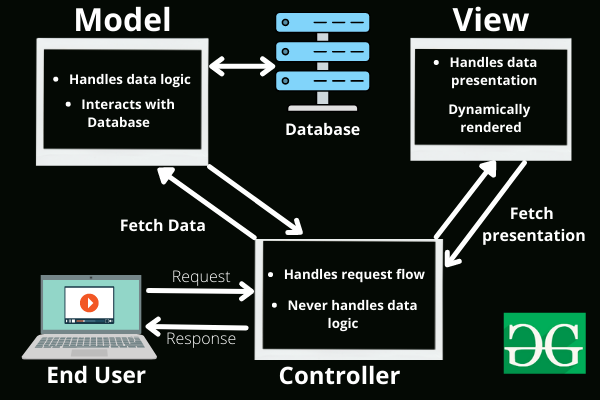
\includegraphics[width=0.9\textwidth]{images/logique.png}
    \caption{Logical architecture}
    \label{fig:logical-architecture}
\end{figure}

Request Flow:
\begin{enumerate}
    \item A user action (e.g., viewing property listings) triggers a request in the frontend.
    \item The request is sent to the backend via an API call.
    \item The Express.js controller processes the request, interacting with the database and other services.
    \item Data is retrieved, processed, and returned as a response.
    \item The frontend updates the UI dynamically based on the received data.
\end{enumerate}

This structured approach ensures a scalable, secure, and high-performance system, optimizing Korpor's real estate investment and management operations.

\section{Work Environment}

In this part, we will talk about our work environment, focusing on different aspects:
our material environment, the techniques we used in the realization of our project as well as the tools we used in our report, the product backlog and sprint planning, and finally, we will conclude this section.

\subsection{Physical environment}

The work was carried out by a laptop computer that is equipped with these detailed features presented in Table \ref{tab:physical-env}:

\begin{table}[htbp]
    \centering
    \begin{tabular}{|l|l|}
        \hline
        \textbf{Computer Name} & MSI \\
        \hline
        \textbf{Processor} & i5 10th gen \\
        \hline
        \textbf{Hard disk} & 512 Go SSD \\
        \hline
        \textbf{RAM} & 24.0 Go \\
        \hline
        \textbf{Operating system} & Windows 11 Pro \\
        \hline
    \end{tabular}
    \caption{Physical environment}
    \label{tab:physical-env}
\end{table}

\subsection{Used technologies}

% Define a command for technology icons to make it easier to adjust if needed
\newcommand{\techicon}[1]{%
  \includegraphics[height=1em]{images/icons/#1.png}%
}

\subsubsection*{\protect\techicon{expo} Expo}

Expo is an open-source platform for making universal native apps for Android, iOS, and the web with JavaScript and React.

\subsubsection*{\protect\techicon{typescript} TypeScript}
                                                                
TypeScript (abbreviated as TS) is a free and open-source high-level programming language developed by Microsoft that adds static typing with optional type annotations to JavaScript. It is designed for the development of large applications and transpiles to JavaScript.

\subsubsection*{\protect\techicon{tanstack} Tanstack}
                                                                      
High-quality open-source software for web developers. Headless, type-safe, \& powerful utilities for Web Applications, Routing, State Management, Data Visualization, Datagrids/Tables, and more.

\subsubsection*{\protect\techicon{clerk} Clerk}
                                                                        
Clerk is a complete suite of embeddable UIs, flexible APIs, and admin dashboards to authenticate and manage your users.

\subsubsection*{\protect\techicon{maestro} Maestro}
                                                                        
Maestro is the simplest, most powerful, and most trusted end-to-end testing platform for mobile and web apps.

\subsubsection*{\protect\techicon{azure} Google cloud platform}

Google cloud platform, or just GCP, is the cloud computing platform developed by Google. It has management, access and development of applications and services to individuals, companies, and governments through its global infrastructure.

\subsubsection*{\protect\techicon{github} GitHub}

GitHub is a platform for developers to build, scale, and deliver secure software.

\subsubsection*{\protect\techicon{express} Express.js}

Express.js is a minimal and flexible Node.js web application framework that provides a list of features for building web and mobile applications easily.

\subsubsection*{\protect\techicon{postman} Postman}

Postman is an API platform for building and using APIs. Postman simplifies each step of the API lifecycle and streamlines collaboration so you can create better APIs—faster.

\subsubsection*{\protect\techicon{vite} Vite}

Vite is a modern build tool that provides a fast and optimized development experience for React 17 applications. It leverages native ES modules and offers a highly efficient development server with hot module replacement (HMR).

\subsubsection*{\protect\techicon{react} React}

React, sometimes referred to as a frontend JavaScript framework, is a JavaScript library created by Facebook.

\subsubsection*{\protect\techicon{mysql} MySQL}

MySQL is the world's most popular open source database. With its proven performance, reliability and ease-of-use, MySQL has become the leading database choice for web-based applications, used by high profile web properties.

\subsubsection*{\protect\techicon{docker} Docker}

Docker is an open platform for developing, shipping, and running applications. Docker enables you to separate your applications from your infrastructure so you can deliver software quickly.

\subsubsection*{\protect\techicon{playwright} Playright}

Playwright is an open-source testing and automation framework that can automate web browser interactions. To put it simply, you can write code that can open a browser.

\subsubsection*{\protect\techicon{storybook} Storybook}

Storybook is a frontend workshop for building UI components and pages in isolation. It helps you develop and share hard-to-reach states and edge cases without needing to run your whole app.

\subsection{Tools used for the report}

% Comment out problematic icon
%\subsubsection*{\protect\techicon{overleaf} Overleaf.com}
\subsubsection*{Overleaf.com}

Overleaf is a collaborative cloud-based LaTeX editor used to write, edit, and publish scientific papers.

% Comment out problematic icon
%\subsubsection*{\protect\techicon{staruml} StarUML}
\subsubsection*{StarUML}

StarUML is a software for creating and editing UML and SysML diagrams. Download the latest version for macOS, Windows or Linux, and see the release notes and supported diagram types.

% Comment out problematic icon
%\subsubsection*{\protect\techicon{canva} Canva}
\subsubsection*{Canva}

Canva is a global company that empowers people to design anything and publish anywhere. Learn about its mission, values, commitments, awards, product, and careers.

\section{Product backlog}

The backlog was created before the sprints to plan the milestones and determine the content of each sprint based on project needs. It includes the following fields:
\begin{itemize}
    \item \textbf{Code:} The unique identifier of the task.
    \item \textbf{Theme:} The subject of a user story.
    \item \textbf{User Story:} A short description of the functionality requested by the client.
    \item \textbf{Priority:} A value indicating the importance of the functionality.
    \begin{itemize}
        \item \textbf{Must:} The feature is essential and must be implemented.
        \item \textbf{Should:} The feature should be implemented if possible.
        \item \textbf{Could:} The feature is optional and may be deprioritized.
        \item \textbf{Won't:} The feature is not a priority at this time.
    \end{itemize}
\end{itemize}

\begin{table}[htbp]
    \centering
    \caption{Korpor Product Backlog}
    \label{tab:product-backlog}
    \begin{tabular}{|c|l|p{8cm}|c|}
        \hline
        \textbf{Code} & \textbf{Theme} & \textbf{User story} & \textbf{Priority} \\
        \hline
        % Add your product backlog items here
        % Example:
        % PB001 & Authentication & As a user, I want to be able to register and login using my email & Must \\
        \hline
    \end{tabular}
\end{table}

\section{Sprint planning}

In order to complete the project within the deadlines set by the internship agreement, planning is an important step in the process. It was therefore necessary to define the essential steps and estimate the time to be devoted to the completion of the various tasks. To do this, we made a GANTT chart.

In our project management, we opted for the proportional distribution method in order to estimate the costs.
Figure \ref{fig:gantt-chart} shows the Gantt chart that describes the progress of our project:

\begin{figure}[htbp]
    \centering
    % Replace with actual image file once available
    % 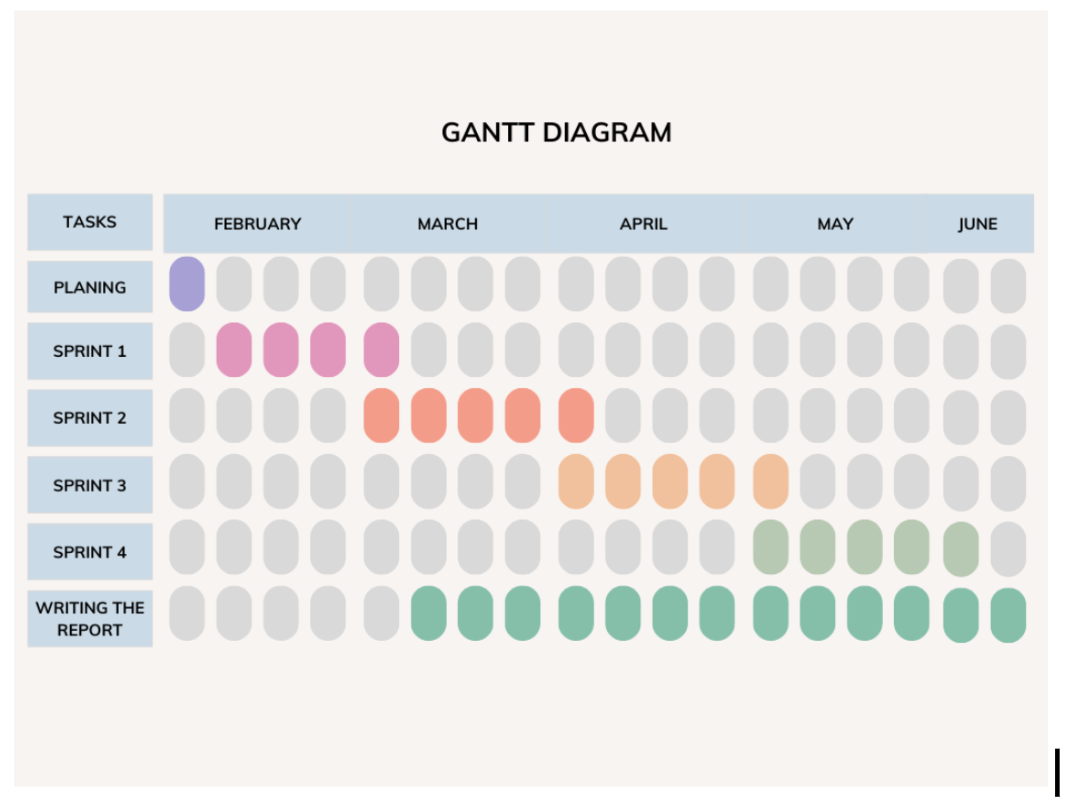
\includegraphics[width=0.9\textwidth]{images/gantt-chart.png}
    \caption{GANTT chart with sprint planning}
    \label{fig:gantt-chart}
\end{figure}

\section{Conclusion}

Our Sprint 0 marked the exciting start of our KORPOR project. We defined global and specific objectives, developed a solid architecture, and configured an optimal working environment. With a clear vision of the initial product backlog and preliminary planning for upcoming sprints, we are ready to achieve our vision and achieve our goals successfully.